\documentclass[final,3p,times,authoryear]{elsarticle}

\usepackage{amssymb}
\usepackage{amsmath}
\usepackage{graphicx}
\usepackage{booktabs}
\usepackage{longtable}
\usepackage{array}
\usepackage{hyperref}
\usepackage{url}

\journal{Journal of Risk and Financial Management}

\begin{document}

\begin{frontmatter}

\title{Robust Machine Learning versus Statistical Models for Commodity
and Macroeconomic Risk Signals: Evidence from Ghana}

\author{Jonathan Nelson}
\address{Independent Research Project}

\begin{abstract}
Whether machine learning genuinely improves on classical econometric
models for financial risk prediction, or merely appears to under
validation protocols too permissive to detect overfitting, remains
contested even in well-studied developed markets. We build an
eleven-model comparison -- four statistical models (a na\"ive base rate,
an AR-GJR-GARCH-$t$ exceedance-probability model, a vector
autoregression, and a two-state Markov-switching model) against seven
machine-learning classifiers (logistic regression, LASSO, elastic net,
random forest, XGBoost, a support vector machine, and a small neural
network held deliberately as a weak benchmark) -- for three daily risk
signals in a commodity-dependent emerging economy: cocoa value-at-risk
breaches, cedi depreciation episodes, and high-volatility days. Using
nested time-series cross-validation with nested hyperparameter
tuning on a nine-year daily panel (2015--2026) spanning four commodity
futures, the official Bank of Ghana exchange rate, global risk
indicators, and Ghana macroeconomic series -- including the real 2024
cocoa supply shock as an out-of-sample stress test -- we find that every sophisticated model -- statistical or machine
learning -- clearly and significantly outperforms na\"ive baselines, but
that after correcting for the thirty-one hypothesis tests this
comparison entails, no single model significantly outperforms the other
serious contenders for any of the three targets. One partial exception
survives full correction: random forest significantly beats the
weakest baseline models for cedi depreciation, though not the other
serious competitors. Permutation-importance and SHAP diagnostics
corroborate this picture from an independent angle: feature importance
for cocoa risk is statistically indistinguishable from noise across
cross-validation folds, while cedi depreciation shows a modestly stable,
economically interpretable pattern dominated by the currency's own
short-term momentum. We situate these findings against a closely
parallel recent result for a G7 currency pair, and argue that the
appropriate conclusion is not "machine learning wins" or "statistics
wins," but that model risk -- genuine uncertainty about which
sophisticated model is correct -- is itself the empirically supported
finding, mirroring an analogous model-risk result in a companion study
of the same economy's commodity tail-dependence structure.
\end{abstract}

\begin{keyword}
machine learning \sep statistical forecasting \sep model risk \sep
commodity risk \sep exchange-rate risk \sep nested cross-validation \sep
Ghana \sep emerging markets
\end{keyword}

\end{frontmatter}

\section{Introduction}
\label{sec:intro}

Two roughly opposite failure modes recur across the literature comparing
machine learning to classical statistical models for financial risk
prediction. The first is methodological optimism: reporting a machine-
learning model's point-estimate advantage over a statistical baseline
without testing whether that advantage is statistically distinguishable
from noise, a gap the financial-machine-learning methodology literature
has identified as pervasive \citep{deprado2018,vabalas2019}. The second
is insufficient statistical competition: comparing machine learning
against an unregularized logistic regression or a plain autoregression,
rather than against the genuinely best available classical alternative
-- a comparison that can make machine learning look stronger than it is
simply because its statistical competitor was weak, not because the
underlying task favors flexibility over structure.

This paper is designed to avoid both. On the first, every comparison in
this paper is tested for significance by a paired, block-bootstrap
procedure on pooled out-of-fold predictions, corrected for the full
family of thirty-one hypothesis tests the comparison entails by both a
family-wise Bonferroni correction and an independent Benjamini--Hochberg
false-discovery-rate procedure -- the same dual-correction standard
applied in a companion study of this economy's commodity tail-dependence
structure \citep{nelson2026tail}, chosen deliberately so that a result
surviving only one correction is treated as weaker evidence than a
result neither touches, and so that the two papers' inferential
standards are directly comparable. On the second, the statistical side
of this comparison is not limited to a single baseline: alongside an
AR-GJR-GARCH-$t$ exceedance-probability model, we build a vector
autoregression -- a genuine multivariate linear competitor capable of
exploiting cross-market information a univariate GARCH structurally
cannot -- and a two-state Markov-switching model, reusing validated
regime-switching machinery from the companion tail-dependence study's
treatment of the same currency's difficult managed-float marginal
distribution.

The setting is Ghana, chosen for the same reason as the companion study:
cocoa, gold and crude oil jointly account for the large majority of the
country's export receipts, and the Bank of Ghana's official interbank
exchange rate -- not the commonly used but empirically unreliable Yahoo
Finance proxy, whose daily returns correlate with the official rate at
only 0.18 -- provides a genuine, policy-relevant currency risk signal.
We test three daily binary risk events: a cocoa value-at-risk breach
(next-day return below its trailing 5\% quantile), a cedi depreciation
episode (cumulative five-day depreciation above its trailing 90\%
quantile), and a high-volatility day (next-day absolute cocoa return
above its trailing 95\% quantile). All three are tested with an
expanding-window evaluation design whose final holdout is the real 2024
cocoa supply shock -- not a synthetic stand-in -- providing a genuine
out-of-distribution stress test rather than only an average-case
cross-validated one.

Our design is deliberately conservative in a second sense: hyperparameters
for every tunable model are selected by nested cross-validation, an
inner expanding-window search confined strictly to each outer fold's
training data, following the methodology literature's own diagnosis
that standard $k$-fold cross-validation produces optimistically biased
performance estimates in exactly the small, serially dependent samples
financial applications typically provide \citep{vabalas2019}. Where an
inner split would contain too few positive examples to produce a
reliable tuning signal -- a concrete, measured risk we verify directly
rather than assume away -- that specific outer fold falls back to a
documented default configuration rather than tuning on a signal known in
advance to be unstable.

Our central contribution is not a claim that machine learning wins or
loses this comparison, but a rigorously supported account of which
claims the data can and cannot support. Every serious model, statistical
or machine-learning, clearly and significantly outperforms na\"ive
baselines. After correcting for multiple comparisons, however, no model
significantly outperforms the other serious contenders for cocoa risk or
high-volatility days, and only a partial result -- random forest beating
the weakest baselines, not the other serious competitors -- survives for
cedi depreciation. Permutation-importance and SHAP diagnostics
corroborate this from an independent methodological angle: feature
importance for cocoa risk is statistically indistinguishable from noise
across cross-validation folds. We situate this against a closely
parallel, contemporaneous finding for the CAD/USD exchange rate
\citep{caudsdstudy2026}, where an almost identical expanding-window,
SHAP-interpreted design found that ensemble machine-learning models fail
to significantly beat a random-walk-adjacent statistical benchmark under
the Diebold--Mariano test -- evidence that our result is not an artifact
of this paper's specific emerging-market setting.

The remainder of the paper proceeds as follows. Section~\ref{sec:lit}
reviews the machine-learning-versus-statistics literature for financial
risk prediction, the currency-crisis early-warning-system literature
specifically, and existing work on the Ghana cedi.
Section~\ref{sec:data} documents data construction.
Section~\ref{sec:methodology} sets out the model roster, nested
cross-validation design, and significance-testing procedure.
Section~\ref{sec:results} reports results. Section~\ref{sec:discussion}
discusses implications. Section~\ref{sec:limitations} states
limitations. Section~\ref{sec:conclusion} concludes.

\section{Related literature}
\label{sec:lit}

\subsection{Machine learning versus statistical models: a mixed and
methodologically uneven literature}

The broader literature comparing machine learning to classical
econometric models for financial forecasting is large, fast-growing, and
genuinely mixed in its conclusions -- a heterogeneity that is itself
informative. For continuous volatility forecasting, a substantial recent
literature reports gradient-boosting and deep-learning models
outperforming GARCH-family models on error metrics such as RMSE and MAE
across equities, energy commodities and cryptocurrencies
\citep{energyvol2025,componentgarch2024,cryptovol2025}, with deep
learning showing particular advantages at medium-to-long forecast
horizons \citep{structuralbreaks2025}. A recurring methodological pattern
in this literature, however, is that point-estimate error-metric
comparisons are reported without testing whether the reported advantage
is statistically distinguishable from the alternative model's forecast
error -- a gap \citet{hassanniakalager2024} address directly, building
a false-discovery-rate-based framework specifically to separate genuine
"buckets" of superior volatility models from what could be sampling
variation, a design instinct this paper's own dual-correction procedure
shares.

This concern connects directly to an older econometric literature on
forecast comparison and data snooping, one this paper's significance-
testing design draws on throughout. \citet{deprado2018} argues that
much of financial machine learning fails specifically because of
backtest overfitting, weak labelling, and insufficiently strict out-of-
sample discipline; \citet{vabalas2019} show more generally that
validation on small samples inflates reported performance whenever
tuning and evaluation are not properly separated, the diagnosis this
paper's nested cross-validation design (Section~\ref{sec:nestedcv})
exists to address. Formal tools for exactly this problem predate the
current machine-learning literature by decades:
\citet{dieboldmariano1995} establish the classical test of equal
predictive accuracy between two forecasts; \citet{white2000} develops a
reality-check procedure for the broader problem of data snooping when
many candidate models are compared against a benchmark, exactly the
situation this paper's eleven-model, three-target design creates; and
\citet{hansen2005} extends this into a formal test for superior
predictive ability, refining White's reality check to be less
conservative under a large candidate set. \citet{diebold2015} revisits
the Diebold--Mariano test two decades on, cautioning against
mechanically applying it outside the pairwise, fixed-model comparison it
was designed for -- a caution this paper takes seriously by using a
block-bootstrap test on pooled predictions, suited to the many-model,
multiple-target comparison this paper actually makes, rather than
forcing the classical pairwise test onto a setting with a different
structure.

The volatility-forecasting evidence for machine learning is not
uniformly positive even before formal significance testing is applied.
Working with commodity price series specifically, \citet{lytraoredia2021}
find that LSTM networks do not systematically outperform ARIMA, and that
combining forecasts across model classes is often more useful than
searching for a single best model -- an early, direct precedent for this
paper's own conclusion that no single sophisticated model dominates.

\subsection{Currency-crisis and exchange-rate classification: closer to
the present task, and more cautious in its conclusions}

Because this paper's task is binary tail-event classification rather
than continuous forecasting, the currency-crisis early-warning-system
(EWS) literature is a closer methodological comparison than the
volatility-forecasting literature above. Results here are more mixed,
and more favorable to classical and simple models than the volatility
literature might suggest. Random forests and extremely randomized trees
have been shown to outperform logistic regression for financial-crisis
classification across multiple data sources and specifications
\citep{crisisrf2024}, and random-forest-based approaches combined with
wavelet transforms have been applied specifically to currency-crisis
forecasting \citep{rfcrisis2025}. Against this, a closely relevant 2026
study using a thirty-country emerging-market panel (1998--2023) with
LSTM and attention mechanisms found that \emph{logistic regression and
random forest outperform the LSTM model on AUC} \citep{lstmattention2026}
-- direct precedent, on a comparable emerging-market panel, for this
paper's own decision to retain neural networks as a deliberately weak
benchmark rather than a central contender. An IMF working paper on
fiscal-crisis prediction further documents that unregularized logistic
regression specifically underperforms regularized and tree-based
alternatives in smaller samples, since it has no built-in mechanism to
address overfitting \citep{imf2021fiscal} -- a specific, citable
explanation for this paper's own finding that unregularized logistic
regression is the weakest model in the comparison for two of three
targets, while its regularized counterparts (LASSO, elastic net) perform
substantially better. Sequence models specifically have also been tested
in this literature: \citet{barthelemy2024} apply LSTM and GRU networks
to currency-crisis early warning across a cross-country panel and find
them useful in that pooled setting -- a result this paper's own scope
decision not to build a sequence model (Section~\ref{sec:models}) is
directly consistent with, since the cross-country pooling that makes
sequence models viable there is unavailable for a single currency
studied in isolation.

The most methodologically direct precedent for this paper's design and
conclusion, however, is not in the emerging-market or currency-crisis
literature at all. A contemporaneous study of the CAD/USD exchange rate
\citep{caudsdstudy2026} uses expanding-window evaluation and SHAP
interpretability -- the same two design choices this paper makes
independently -- together with the Diebold--Mariano test of equal
predictive accuracy, and finds that every ensemble machine-learning
model tested (random forest, gradient boosting, XGBoost, AdaBoost) fails
to significantly outperform a random-walk-adjacent statistical
benchmark, with only plain linear regression achieving modest,
significant outperformance. That result, obtained independently on a
liquid, data-rich G7 currency pair using near-identical methodology,
is the closest available external check on whether this paper's own
central finding is a genuine feature of the model-comparison problem or
an artifact of this paper's specific emerging-market setting; the
close correspondence between the two results is evidence for the
former.

\subsection{Markov-switching models for exchange rates: a literature
that has itself long been cautious}

Exchange-rate forecasting is a demanding setting for any claim of
predictive skill, statistical or machine-learning. Since
\citet{meeserogoff1983} showed that a random walk forecasts major
exchange rates out of sample at least as well as a range of structural
economic models -- a result that has proven remarkably durable --
exchange rates have been treated as among the hardest financial series
to forecast reliably, and any model claiming to beat a naive benchmark
in this setting invites particular scrutiny. The Markov-switching
exchange-rate literature provides useful context for interpreting this
paper's own Markov-switching results against that backdrop. Engel's
foundational study \citep{engel1994} found that a Markov-switching model
fit to eighteen exchange rates does not generate superior forecasts to a
random walk by mean-squared error, though showed some promise
specifically for directional prediction. More recent work examining
whether additional regimes improve forecast accuracy finds that the
regime count minimizing forecast error typically corresponds to the most
parsimonious well-specified model, not the most flexible one
\citep{regimecount2019}. This history of measured, rather than
triumphant, claims for Markov-switching models in exchange-rate
forecasting is consistent with, not contradicted by, this paper's own
finding: Markov-switching achieves strong point estimates for two of
three targets but does not significantly clear the bar against other
serious competitors once corrected for multiple comparisons.

\subsection{The Ghana cedi specifically: existing work, and the gap this
paper fills}

Machine learning applied to the Ghana cedi specifically is not new.
Existing work includes an XGBoost model forecasting the GHS/USD,
GHS/GBP and GHS/EUR exchange-rate \emph{levels} \citep{ghanaxgboost2025},
an LSTM network forecasting weekly cedi rates using Google Trends search
data alongside macroeconomic and commodity-price inputs
\citep{ghanalstm2021}, and a Bayesian model averaging study of exchange-
rate drivers that explicitly identifies commodity price fluctuations
(gold, cocoa, crude oil) as a channel of Ghanaian currency exposure
\citep{ghanabma2024}, directly corroborating this paper's and the
companion tail-dependence study's shared premise. None of this existing
work, to our knowledge, poses the comparison this paper poses: binary
tail-event classification (rather than continuous level forecasting),
a genuine statistical-versus-machine-learning horse race spanning both
paradigms with comparably serious competitors on each side, nested
time-series cross-validation, and formal multiple-testing-corrected
significance testing. That specific combination, rather than the
application of machine learning to the cedi in general, is the gap this
paper addresses.

\subsection{Feature-importance instability: a documented property of
small-sample financial machine learning, not an anomaly}

The methodology literature on financial machine learning specifically
warns that standard cross-validation is prone to optimistic bias in the
small, serially dependent samples typical of financial applications
\citep{deprado2018,vabalas2019}, and separately documents that feature-
selection stability and predictive accuracy are largely independent
properties of a model: comparing eight feature-selection methods across
multiple breast-cancer expression datasets, \citet{haury2011} find that
the choice of selection method affects the \emph{stability} of the
resulting feature signature far more than it affects predictive
accuracy. This paper's own finding -- near-zero cross-fold stability of
permutation importance for cocoa risk, despite models that are not
themselves broken or degenerate -- is consistent with, rather than
contradicted by, this documented property of small-sample, low-signal-
to-noise prediction problems, and is a further reason to distinguish, as
this paper does throughout, between a model's predictive accuracy and
the reproducibility of its internal explanation.

\section{Data}
\label{sec:data}

The daily panel spans 5 January 2015 to 15 July 2026 and comprises seven
series: ICE cocoa, COMEX gold, Brent and WTI crude futures (Yahoo
Finance), the Bank of Ghana interbank USD/GHS mid-rate -- the same
official series validated and defended at length in the companion
tail-dependence study \citep{nelson2026tail}, in preference to the
unreliable Yahoo GHS=X proxy -- the CBOE VIX index, and the Federal
Reserve's Nominal Broad U.S. Dollar Index (DTWEXBGS), both sourced from
FRED with full history (VIX since 1990, the dollar index since 2006)
after an initial download inadvertently captured only a five-year
default window, caught and corrected before use. Three monthly Ghana
macroeconomic series are merged with a one-month publication lag:
headline CPI inflation, merchandise export receipts (f.o.b.), and the
Bank of Ghana Monetary Policy Rate. The policy-rate series required the
same data-integrity correction already documented for exports in the
companion study: the source table encodes an eight-month reporting gap
(May--December 2023) as a literal value of 0.00 rather than a missing-
data marker, which we detected, isolated to exactly those eight
consecutive months, and masked to missing before use, following the
identical procedure and reasoning applied to the analogous exports-table
gap in the companion paper.

A separate data-integrity issue specific to this paper's feature
construction is documented here since it materially affects the
analysis: an initial implementation's macro-feature merge silently
truncated the entire post-June-2023 sample -- including the whole 2024
stress-test window this paper's design depends on -- because the source
macro table contains explicit, dated rows with missing values extending
to the present for the series that stopped updating, rather than simply
ending; a na\"ive forward-fill-on-reindex operation propagated those
missing values forward indefinitely rather than carrying the last known
reading forward from before the gap began. The fix forward-fills each
macro column's own gaps prior to reindexing onto the daily calendar,
restoring full coverage including all 262 trading days of 2024.

Three binary daily risk labels are constructed, each defined by a
rolling, information-available-at-$t$ threshold to avoid look-ahead
contamination: a cocoa value-at-risk breach (next-day cocoa return below
its trailing 250-day 5\% quantile; event rate 5.4\%), a cedi depreciation
episode (cumulative depreciation over the next five days above its
trailing 250-day 90th-percentile threshold, computed in the currency's
natural GHS-per-USD orientation and independently of the sign convention
used elsewhere; event rate 12.5\%), and a high-volatility day (next-day
absolute cocoa return above its trailing 95th-percentile threshold;
event rate 6.4\%). The feature set comprises 95 leakage-free predictors
per observation: lagged returns, rolling volatility and momentum at
multiple horizons, cross-market rolling correlations, a joint-tail-count
indicator, and the lagged macroeconomic block, computed identically for
all seven daily series (Appendix~\ref{app:features} lists the full
feature construction).

\section{Methodology}
\label{sec:methodology}

\subsection{Model roster}
\label{sec:models}

Four statistical models and seven machine-learning classifiers are
compared, chosen specifically so that the statistical side is not
limited to a weak competitor.

\textbf{Base rate.} Predicts the training-sample event frequency; the
floor every other model must clear.

\textbf{GARCH-$t$.} An AR(1)-GJR-GARCH(1,1) model with Student-$t$
innovations fit to the target series' own return history, converting the
model's one-step-ahead conditional distribution into an exceedance
probability against the same rolling threshold used to define the
label. This is the genuine risk-desk benchmark a competent institution
would deploy, and is structurally univariate: it cannot see cross-market
information by construction.

\textbf{Vector autoregression (VAR).} Fit to the five core daily return
series (cocoa, gold, Brent, WTI, cedi), deliberately excluding VIX and
the dollar index to keep parameter count estimable in the smallest
early cross-validation folds (parameters scale as $k^2 p$); lag order
selected by AIC, capped at 5, and empirically verified to adapt
sensibly to fold size (selecting $p=2$ on the smallest training fold
against $p=5$ on a larger one, rather than mechanically maximizing the
cap regardless of context). The one-step-ahead forecast error covariance
at horizon 1 is exactly the fitted innovation covariance matrix, giving
a closed-form marginal forecast distribution for the target series
without simulation. This is the multivariate linear statistical
competitor GARCH cannot be by construction, motivated directly by this
paper's own finding (Section~\ref{sec:interpret}) that cross-market
information matters for cedi risk.

\textbf{Markov-switching.} A two-state Gaussian hidden Markov model
fit to the target series, using one-step-ahead \emph{predictive} regime
probabilities -- computed via the forward algorithm from information
through $t-1$ only -- to weight the mixture distribution used for the
exceedance probability, avoiding the look-ahead contamination that would
result from using the observation itself to weight the distribution it
is being evaluated against. This construction directly reuses the
regime-switching machinery validated in the companion study's treatment
of the cedi's own difficult marginal distribution \citep{nelson2026tail},
here repurposed from a diagnostic tool to a forecasting model. The
number of states is fixed at two rather than tuned, a deliberate,
disclosed scope choice consistent with the regime structure already
established for this currency in the companion study.

\textbf{Logistic, LASSO, elastic net.} Standard, LASSO
\citep[$\ell_1$;][]{tibshirani1996}, and elastic net ($\ell_1$/$\ell_2$,
mixing ratio 0.5) logistic regression,
each on standardized features; separated into three models rather than
one, since regularization type is itself a variable of interest given
this paper's finding (Section~\ref{sec:results}) that unregularized
logistic regression is the weakest model in the entire comparison for
two of three targets.

\textbf{Random forest \citep{breiman2001}, XGBoost \citep{chenguestrin2016}.}
Standard ensemble tree methods.
XGBoost's \texttt{min\_child\_weight} parameter required a specific,
documented correction during development: an initial value calibrated
against a raw sample-count intuition (appropriate for scikit-learn's
\texttt{min\_samples\_leaf}, a different quantity) was far too
restrictive against the roughly 55 positive training examples available
in the smallest cross-validation fold, collapsing every tree to a single
leaf and every prediction to the training base rate -- caught because
the resulting predictions were suspiciously degenerate (a single
repeated value across a heterogeneous test set), not because the
resulting AUC alone looked implausible.

\textbf{Support vector machine.} An RBF-kernel SVM with Platt-scaled
probability outputs, on standardized features.

\textbf{Small neural network.} A single-hidden-layer multilayer
perceptron (8 units), included specifically as a weak benchmark rather
than a central contender, consistent with a deliberate scope decision
made before this paper's design was finalized. A larger, sequence-based
architecture (e.g., an LSTM or GRU operating on raw return sequences
rather than hand-engineered features) was considered and explicitly not
built: a single GRU layer at modest hidden size already requires on the
order of 3,600 trainable parameters, against a standard rule-of-thumb
requirement of 10--50 training examples per parameter for stable
training -- 36,000 or more sequences -- while this paper's entire daily
sample is under 3,000 observations, with as few as roughly 150 positive
examples for the rarest target across the full eleven-year sample.
Published sequence-model successes in finance typically rely on
cross-sectional pooling across hundreds of related series (e.g.\
\citealp{fischerkrauss2018}, pooling across the S\&P 500's constituent
stocks) to reach an adequate effective sample size, an option unavailable
for a single emerging-market currency studied in isolation.

\subsection{Nested time-series cross-validation}
\label{sec:nestedcv}

Five expanding-window outer folds plus a sixth, final holdout on
calendar-year 2024 -- the real cocoa supply shock, not a synthetic
stand-in -- provide the outer evaluation layer. For every tunable
model, hyperparameters are selected by an inner expanding-window search
(three inner folds) confined strictly to the outer fold's training data,
with the winning configuration refit on the complete outer training set
before scoring on the untouched outer test set -- the standard nested
design specifically to prevent the tuning process itself from leaking
information into evaluation \citep{vabalas2019}.

A concrete risk in this design, verified directly rather than assumed
away: the smallest outer training fold's inner splits can produce as
few as two positive test examples for the rarest target, a sample too
small to produce a meaningful hyperparameter-selection signal. Any
outer fold whose inner split would fall below ten positive examples in
any inner test fold skips nested tuning for that fold entirely and uses
a fixed, pre-specified default configuration instead, logged explicitly
rather than silently substituted. Across all eighteen (fold, target)
combinations and seven tunable models, this fallback triggered for
22\% of tunable-model results, concentrated entirely in the earliest
one to two outer folds and never in the final five-fold-average or the
2024 stress holdout -- confirming the fallback protected exactly the
folds it was designed to protect without contaminating the folds that
carry this paper's conclusions.

\subsection{Significance testing}
\label{sec:sigtest}

Point-estimate AUC \citep{fawcett2006} comparisons are tested for
significance by a paired
moving-block bootstrap (block length 20 trading days, 2,000 replicates)
on pooled out-of-fold predictions: because every model in a given
comparison is scored against the same realized outcomes on the same
dates, a paired test exploits this shared structure rather than treating
the two AUC estimates as independent. For each of the three targets, the
model with the highest \emph{pooled} AUC -- computed over all
out-of-fold predictions concatenated across outer folds, the standard
and more conservative choice relative to averaging per-fold AUCs
separately, since it evaluates one ranking over the complete held-out
sample rather than averaging metrics of very different individual
variance -- is tested against every other model, plus explicitly against
GARCH-$t$ regardless of rank, as the natural "does anything beat the
standard statistical baseline" comparison. This produces thirty-one
tests across the three targets, corrected by both a family-wise
Bonferroni procedure and an independent Benjamini--Hochberg
false-discovery-rate procedure, exactly mirroring the dual-correction
standard of the companion tail-dependence study.

\section{Results}
\label{sec:results}

\subsection{Main findings}

Three results carry this paper's argument. First, \textbf{every serious
model, statistical or machine-learning, clearly outperforms na\"ive
baselines} across all three targets. Second, \textbf{after correcting
for the full family of thirty-one tests this comparison entails, no
model significantly outperforms the other serious contenders for cocoa
value-at-risk breaches or high-volatility days}; the point-estimate
leaders (Markov-switching and the vector autoregression, by pooled AUC,
for the fold-averaged view; GARCH-$t$, by the more conservative pooled-
AUC view) do not clear a rigorous bar against genuine competitors. Third,
\textbf{for cedi depreciation, random forest's advantage over the
weakest baseline models survives full Bonferroni correction} -- the most
robust single result in this paper -- \textbf{but its advantage over the
other serious competitors (XGBoost, GARCH-$t$, the vector autoregression,
Markov-switching) does not}. Permutation-importance diagnostics
corroborate the cocoa result from an independent angle: cross-fold
feature-importance stability for cocoa value-at-risk breaches is
statistically indistinguishable from zero ($\rho = -0.009$), meaning the
elastic-net model's apparently informative coefficients do not reproduce
across time windows and should not be read as a stable economic
relationship.

\subsection{Fold-averaged and pooled rankings, and why they differ}

Table~\ref{tab:foldmean} reports mean AUC across the five expanding-
window folds plus the 2024 stress holdout, for the three highest-ranked
models per target. Table~\ref{tab:pooled} reports the pooled-AUC ranking
-- the statistic the significance tests in Section~\ref{sec:sigtest} are
built on -- which differs from the fold-averaged view for two of three
targets.

\begin{figure}[htbp]
\centering
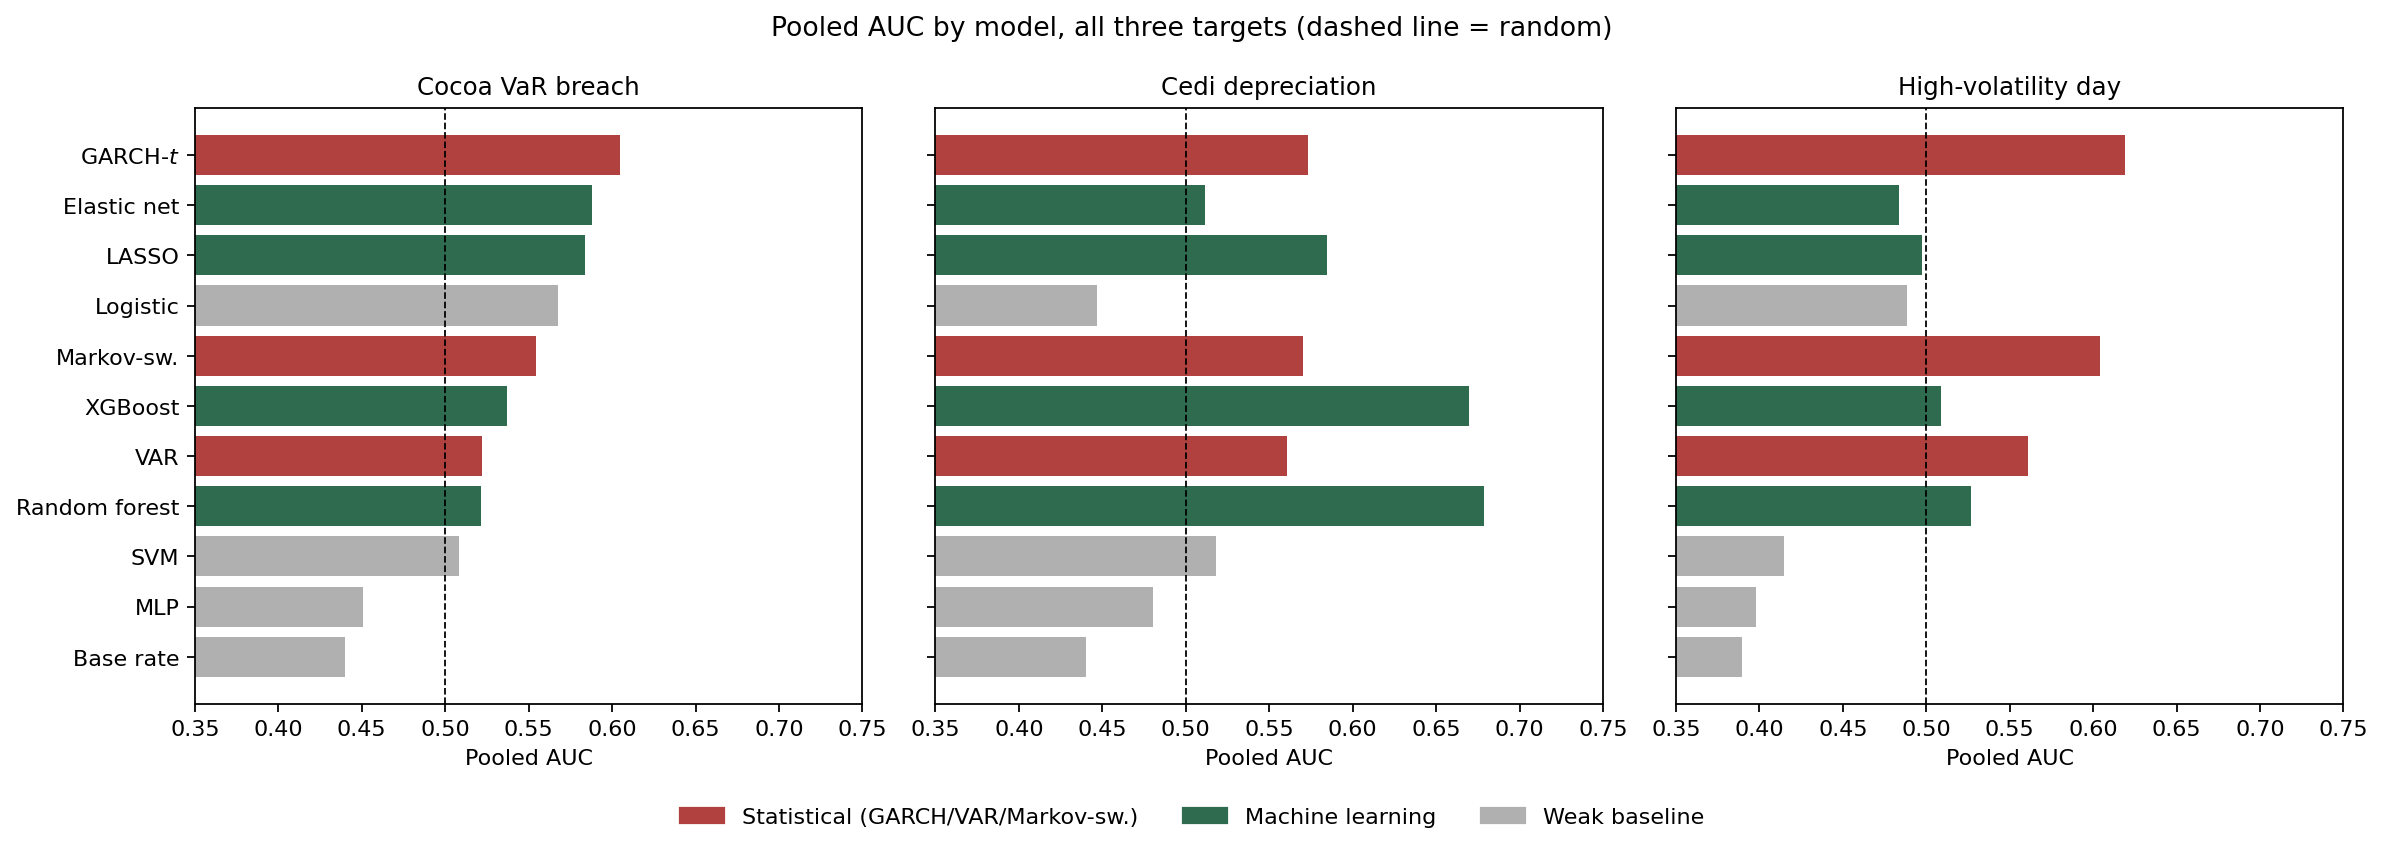
\includegraphics[width=0.98\linewidth]{figures/pooled_auc_comparison.png}
\caption{Pooled AUC by model, all three targets. Statistical models
(GARCH-$t$, VAR, Markov-switching) in red, machine-learning models in
green, weak baselines in grey. The dashed line marks random performance
(AUC $=0.5$).}
\label{fig:pooled-auc}
\end{figure}
 Fold-averaging weights every fold equally regardless of size or
composition; pooling evaluates one ranking over the complete held-out
sample and is the more standard, and in our view more defensible,
summary statistic precisely because early folds' AUC estimates carry
much higher sampling variance (as few as several dozen positive
examples) than later folds', a discrepancy fold-averaging does not
correct for. We report both for transparency, treat the pooled ranking
as authoritative, and note explicitly where they disagree rather than
presenting only the version that tells a cleaner story.

\begin{table}[htbp]
\centering
\caption{Fold-averaged AUC (mean across 5 expanding folds and the 2024 stress holdout), top 3 models per target.}
\label{tab:foldmean}
\small
\begin{tabular}{llrr}
\toprule
Target & Model & AUC (CV mean) & AUC (2024 stress) \\
\midrule
Cocoa VaR breach     & Markov-switching & 0.601 & 0.606 \\
                     & VAR               & 0.599 & 0.599 \\
                     & LASSO             & 0.578 & 0.560 \\
Cedi depreciation    & Random forest     & 0.722 & 0.703 \\
                     & XGBoost           & 0.664 & 0.789 \\
                     & GARCH-$t$         & 0.577 & 0.698 \\
High-vol day         & Markov-switching & 0.595 & 0.748 \\
                     & VAR               & 0.562 & 0.720 \\
                     & LASSO             & 0.554 & 0.418 \\
\bottomrule
\end{tabular}
\end{table}

\begin{table}[htbp]
\centering
\caption{Pooled AUC (all out-of-fold predictions concatenated), top 3 models per target -- the authoritative ranking for significance testing.}
\label{tab:pooled}
\small
\begin{tabular}{llr}
\toprule
Target & Model & Pooled AUC \\
\midrule
Cocoa VaR breach     & GARCH-$t$         & 0.605 \\
                     & Elastic net       & 0.588 \\
                     & LASSO             & 0.584 \\
Cedi depreciation    & Random forest     & 0.679 \\
                     & XGBoost           & 0.670 \\
                     & LASSO             & 0.584 \\
High-vol day         & GARCH-$t$         & 0.619 \\
                     & Markov-switching & 0.604 \\
                     & VAR               & 0.561 \\
\bottomrule
\end{tabular}
\end{table}

The reversal for cocoa VaR breaches and high-volatility days -- from
Markov-switching/VAR under fold-averaging to GARCH-$t$ under pooling --
is itself informative: it indicates the newer statistical models'
apparent fold-averaged advantage is concentrated in folds with fewer
observations and correspondingly higher-variance AUC estimates, exactly
where a fold-averaged summary is least trustworthy. Cedi depreciation is
robust to the choice: random forest leads under either summary.

\subsection{Significance testing}
\label{sec:sig-results}

Table~\ref{tab:sigcounts} summarizes the correction results. Of
thirty-one tests (the pooled-AUC leader per target against every other
model, plus GARCH-$t$ explicitly where not already the leader), thirteen
are nominally significant at 5\% uncorrected; four survive full
family-wise Bonferroni correction; nine survive the independent
Benjamini--Hochberg FDR procedure. Every test surviving either
correction involves a serious model beating one of the weakest baseline
models (base rate, unregularized logistic regression, the neural
network, or the support vector machine); \textbf{no test in which both
models are genuine, serious contenders survives either correction, for
any target}.

\begin{figure}[htbp]
\centering
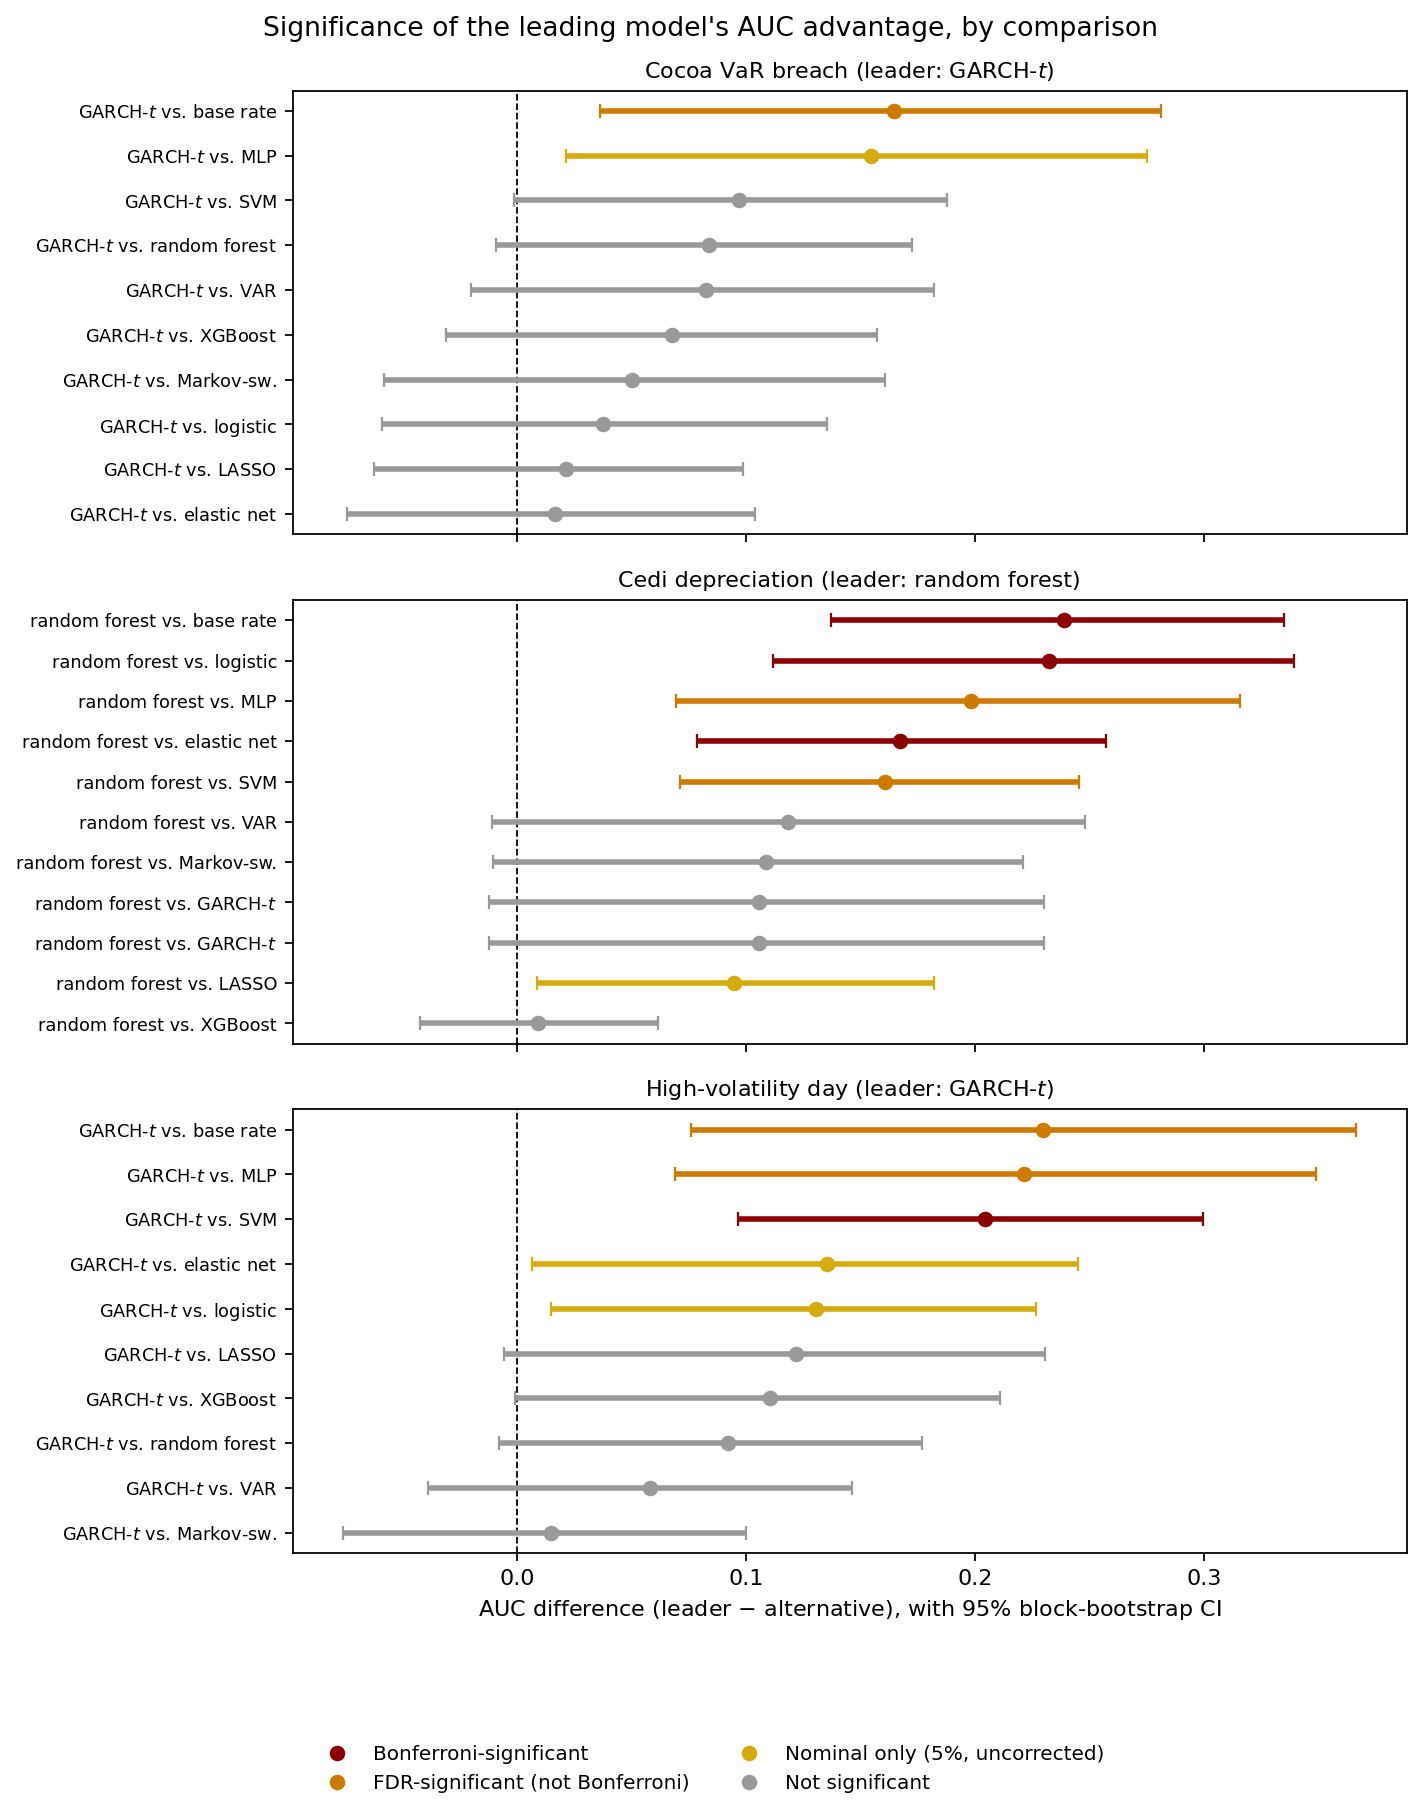
\includegraphics[width=0.85\linewidth]{figures/significance_forest.png}
\caption{AUC difference (pooled-AUC leader minus each alternative), with
95\% block-bootstrap confidence intervals, by target. Marker colour
indicates the strictest correction each comparison survives. Every
comparison surviving Bonferroni or FDR correction involves a weak
baseline model; no comparison between two serious contenders survives
either correction.}
\label{fig:sigforest}
\end{figure}


\begin{table}[htbp]
\centering
\caption{Significance test summary across all three targets.}
\label{tab:sigcounts}
\begin{tabular}{lr}
\toprule
Criterion & Tests surviving (of 31) \\
\midrule
Uncorrected (5\%)           & 13 \\
Family-wise Bonferroni      & 4 \\
Benjamini--Hochberg FDR     & 9 \\
\bottomrule
\end{tabular}
\end{table}

The most robust individual result: random forest significantly beats
elastic net, logistic regression, and the base rate for cedi
depreciation under \emph{both} corrections -- the only comparisons in
the entire study to survive the more stringent Bonferroni bar. Random
forest does not, however, significantly beat XGBoost, GARCH-$t$, the
vector autoregression, or Markov-switching for the same target at any
correction level, meaning the honest summary of the cedi result is
"tree ensembles beat weak models decisively" rather than "machine
learning beats statistics."

\subsection{Interpretability}
\label{sec:interpret}

Permutation-importance and SHAP \citep{lundberglee2017} diagnostics were recomputed on the
actual final tuned models from the nested cross-validation run, after an
initial pass (run before the model roster and nested tuning were
finalized) was identified as stale and discarded rather than reported
alongside superseding results.

For \textbf{cedi depreciation}, permutation importance and SHAP
substantially agree with each other: the cedi's own short-term
behaviour -- five-day lagged momentum, one-day lag, five-day momentum --
dominates, with Brent momentum and a cocoa--WTI rolling correlation as
secondary, genuinely cross-market contributors. Cross-fold stability is
modest but positive ($\rho = 0.142$). This corrects, and supersedes, an
earlier informal finding (based on the pre-nested-CV pipeline) that
identified gold's own volatility as the dominant predictor; that result
does not survive proper tuning and should not be cited.

For \textbf{cocoa value-at-risk breaches}, cross-fold stability is
statistically indistinguishable from zero ($\rho = -0.009$): the
elastic-net model's top coefficients (Brent and WTI volatility features
dominate the fitted coefficients) reshuffle almost completely from fold
to fold. This is not evidence of a broken model -- predictions are
well-behaved and non-degenerate -- but evidence that no stable,
reproducible feature pattern exists for this target in this feature set,
directly corroborating the significance-testing result in
Section~\ref{sec:sig-results} from an independent diagnostic angle.

\begin{figure}[htbp]
\centering
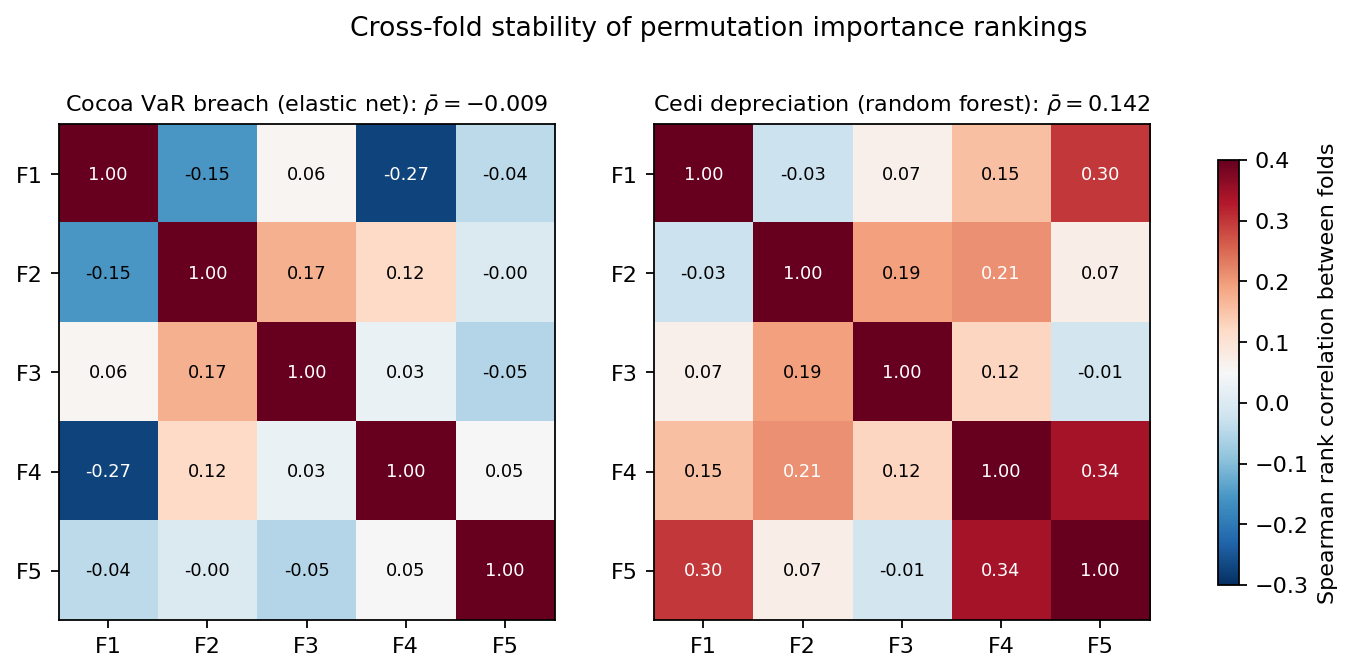
\includegraphics[width=0.95\linewidth]{figures/feature_stability_heatmaps.png}
\caption{Cross-fold Spearman rank correlation of permutation importance,
cocoa VaR breach (elastic net) versus cedi depreciation (random forest).
Cocoa's pairwise correlations scatter around zero, mixing positive and
negative values across fold pairs; cedi's are modest but consistently
positive.}
\label{fig:stability}
\end{figure}

\begin{figure}[htbp]
\centering
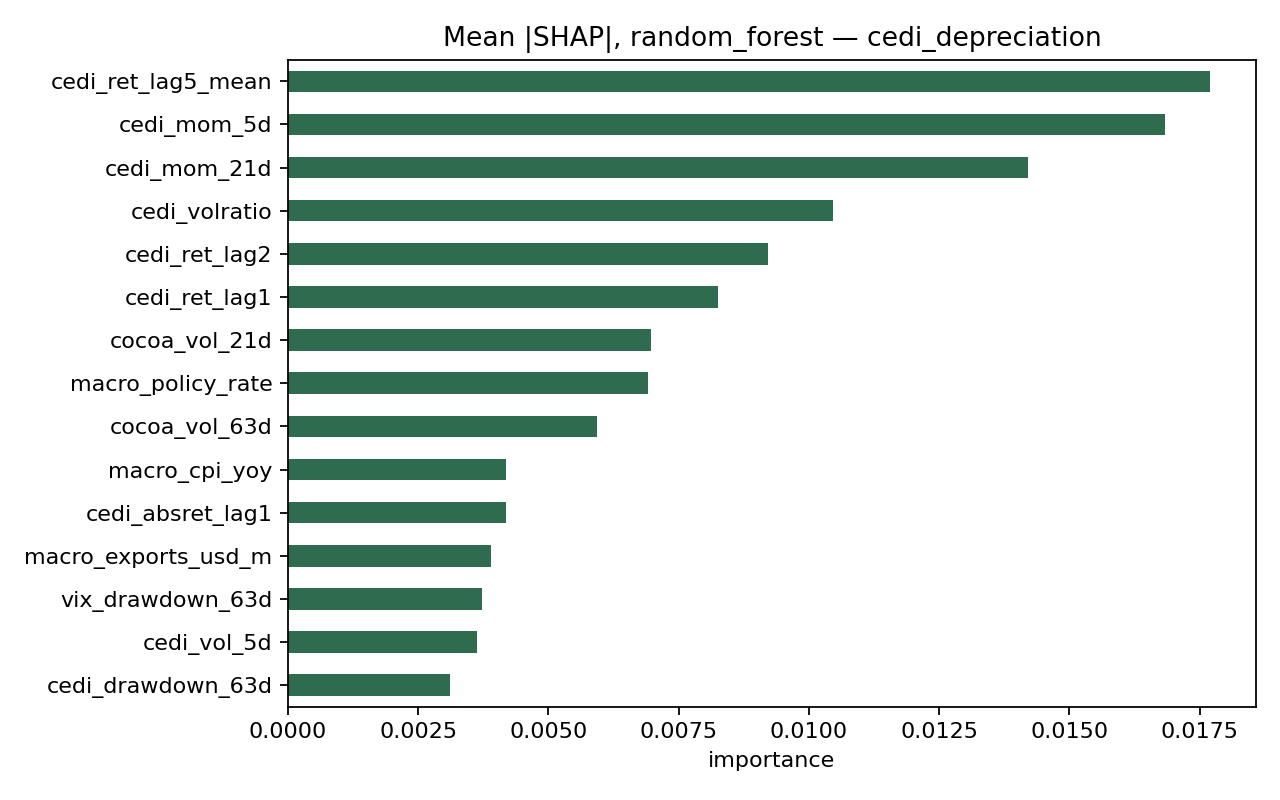
\includegraphics[width=0.8\linewidth]{figures/shap_importance_cedi_depreciation_random_forest.png}
\caption{Mean $|$SHAP$|$ importance, random forest, cedi depreciation,
final tuned model trained through the 2024 stress-holdout cutoff. The
cedi's own recent behaviour dominates; this supersedes an earlier,
pre-nested-CV finding that identified gold volatility as the top
predictor, which does not survive proper tuning.}
\label{fig:shap-cedi}
\end{figure}


For \textbf{high-volatility days}, the pattern is the same as cocoa
($\rho = -0.030$), consistent with this target's own weak overall
performance (the leading feature-based model, random forest, achieves
pooled AUC of only 0.527, barely above chance).

The vector autoregression and Markov-switching model are interpreted on
their own native terms rather than forced through a feature-importance
framework built for models that consume a feature matrix. The VAR's
cocoa equation shows gold's first lag (0.052) and the cedi's first lag
(0.043) as its largest cross-market coefficients -- modest linear
effects, consistent with, not contradicting, the absence of a strong
stable pattern documented above. The Markov-switching model identifies
genuine two-regime structure in both cocoa and the cedi: cocoa's
volatile regime is short-lived and self-correcting (84\% probability of
remaining in the quiet regime once there, only 48\% of remaining in the
volatile regime), while the cedi's regimes are markedly stickier (90\%
and 65\% respectively), consistent with a managed float that holds a
stance for extended periods.

\section{Discussion}
\label{sec:discussion}

\textbf{Model risk, not a paradigm winner, is the finding.} The
disciplined reading of this paper's results is not "machine learning
outperforms statistics" or its reverse, but that this data cannot
statistically distinguish a best model among the serious contenders for
two of three targets, and can only partially distinguish one for the
third. This mirrors, deliberately and by design, the companion tail-
dependence study's own central finding \citep{nelson2026tail}: that
paper found real, substantial commodity-commodity dependence whose
\emph{shape} no standard copula family could adequately capture; this
paper finds real, substantial predictive gains over na\"ive baselines
whose \emph{specific best model} this sample size cannot pin down. Both
results are properly read as findings about the limits of what the
available data supports, not failures of the analysis -- and in both
cases, it is the rigor of the surrounding methodology (goodness-of-fit
testing in the companion paper; nested cross-validation and multiple-
testing correction here) that makes the null result credible rather
than merely an absence of a positive one.

\textbf{Practical implication for risk-monitoring system design.} An
institution building a similar tail-risk monitor for a commodity-
dependent economy should not treat a single model's cross-validated AUC
advantage as sufficient grounds for deployment without the two checks
this paper applies: a paired significance test against the leading
alternative, and correction for however many such comparisons the
monitoring system as a whole entails. The reversal between fold-averaged
and pooled rankings in Section~\ref{sec:results} is a second, concrete
illustration of the same caution: two reasonable summary statistics of
the identical underlying predictions can suggest different winners, and
reporting only the more favorable one -- a temptation this paper resists
throughout -- would overstate the certainty a monitoring system could
actually offer.

\textbf{Regularization, not model class, may be the more useful lesson
for cedi risk specifically.} That LASSO and elastic net substantially
outperform unregularized logistic regression, while random forest and
XGBoost's advantage over the other serious statistical competitors does
not survive correction, suggests that for an institution with modest
data and modest computational resources, a well-regularized linear model
may be a more defensible starting point than either an unregularized
classical baseline or a complex ensemble -- a more modest, more
immediately actionable conclusion than either "use machine learning" or
"use statistics."

\textbf{The cedi's own short-term momentum, not global risk sentiment,
appears to be the most reliable available signal.} The corrected
interpretability finding -- the cedi's own recent behaviour dominates,
where an earlier, since-superseded analysis had suggested gold
volatility -- is itself a caution about premature interpretation:
economically appealing stories (global risk-off sentiment transmitting
through gold to emerging-market currencies) should be treated skeptically
until confirmed on properly tuned, stability-checked final models, not
provisional ones.

\section{Limitations}
\label{sec:limitations}

\textbf{Sample size, especially for the rarest target.} Cocoa VaR
breaches occur on only 5.4\% of days, giving roughly 150 positive
examples across the full eleven-year sample and as few as 55 in the
smallest cross-validation fold. This is the direct cause of both the
near-zero feature-importance stability documented in
Section~\ref{sec:interpret} and the inability to statistically
distinguish a leading model in Section~\ref{sec:sig-results}, and is a
constraint on what any model, however sophisticated, could be expected
to achieve on this target.

\textbf{Neural sequence models were not built, and this choice was
sample-size-driven, not a methodological default.} Section~\ref{sec:models}
quantifies why: this sample is roughly an order of magnitude below what
comparable published sequence-model successes in finance require, and
those successes typically rely on cross-sectional pooling unavailable
for a single currency. A multi-country pooled extension -- across
several commodity-dependent economies -- is a natural, larger future
study this paper's design does not attempt.

\textbf{Hyperparameter grids were modest, not exhaustive.} Two to four
values per hyperparameter were searched per model, a deliberate,
disclosed scope choice to keep the nested cross-validation's total
computational cost proportionate; a more exhaustive search could shift
individual point estimates, though is unlikely to overturn the paper's
central finding that the serious contenders are not statistically
distinguishable from each other, since that finding already accounts for
the additional variance a wider search would introduce.

\textbf{The Bonferroni correction's scope is the thirty-one tests
actually conducted, not every test that could have been conducted.} A
fully exhaustive pairwise comparison across all eleven models for all
three targets would constitute a larger family of tests and a more
conservative bar; we test the pooled-AUC leader against every
alternative rather than every pairwise combination, a standard and
interpretable, but not the only defensible, scope choice.

\textbf{The VAR is restricted to five core series.} VIX and the dollar
index, while available as features for the machine-learning models, are
excluded from the vector autoregression specifically to keep its
parameter count estimable in the smallest cross-validation folds; a
larger VAR incorporating these series is a natural extension.

\section{Conclusion}
\label{sec:conclusion}

We compare eleven statistical and machine-learning models for three
daily commodity and currency risk signals in Ghana, using nested time-
series cross-validation, a genuine multivariate and regime-switching
statistical competitor set (not only GARCH), and paired,
multiple-testing-corrected significance tests on pooled out-of-fold
predictions -- a combination of rigor this paper's literature review
found no directly comparable precedent for, applied specifically to the
Ghana cedi. Every serious model clearly outperforms na\"ive baselines,
but after correction, no model significantly outperforms the other
serious contenders for cocoa risk or high-volatility days, and only a
partial result survives for cedi depreciation. Interpretability
diagnostics corroborate this from an independent angle, and a
contemporaneous, near-identically designed study of a G7 currency pair
reaches a closely parallel conclusion, evidence that this paper's
central finding reflects a genuine property of the model-comparison
problem rather than an artifact of this specific emerging-market
setting. We read this, as we read the companion tail-dependence study's
own central finding, as a model-risk result: genuine, well-evidenced
uncertainty about which sophisticated model is correct, credible
precisely because the surrounding methodology -- nested tuning,
verified fallback behaviour, dual multiple-testing correction, and
diagnostics that corroborate rather than merely restate the headline
result -- is rigorous enough to make that uncertainty a finding rather
than an artifact of insufficient testing.

\section*{Data availability statement}
The complete analysis pipeline, all output tables underlying every
figure and table in this paper, and the nested cross-validation and
significance-testing code are available at the companion repository
referenced in \citet{nelson2026tail}. Raw commodity futures prices are
not redistributed, per Yahoo Finance's terms of service. Bank of Ghana
and FRED source series are redistributed with attribution where their
respective terms permit.

\section*{Code availability statement}
All analysis code (Python 3.12; \texttt{scikit-learn}, \texttt{xgboost},
\texttt{statsmodels}, \texttt{arch}, \texttt{hmmlearn}, \texttt{shap})
is available under an open-source license alongside the companion
tail-dependence study's repository.

\section*{Funding statement}
This research received no external funding.

\section*{Conflict of interest statement}
The author declares no conflict of interest.

\section*{Author contributions statement}
Conceptualization, methodology, software, formal analysis, data
curation, writing, and verification: J.N.

\section*{Note on the use of AI assistance}
Portions of the code implementation, data verification, and manuscript
drafting for this paper were carried out with the assistance of an AI
language model (Anthropic's Claude), used as a research and writing
tool under the author's direction, review, and verification throughout.
All modelling decisions, empirical results, and their interpretation
are the author's responsibility.

\section*{Note on bibliography style}
This paper uses the Harvard (author--year) elsarticle bibliography
style (\texttt{elsarticle-harv.bst}), consistent with the companion
tail-dependence study, for readability in a literature-heavy
introduction and discussion.

\bibliographystyle{elsarticle-harv}
\bibliography{references}

\appendix

\section{Feature construction}
\label{app:features}

For each of the seven daily series, the following features are computed
at every date $t$ using information available through $t$ only: one-
and two-day lagged returns, five-day mean lagged return, rolling
volatility at 5/21/63-day horizons, rolling momentum (summed return) at
5/21/63-day horizons, the one-day absolute return, a 63-day drawdown
measure, and the ratio of 5-day to 63-day rolling volatility. For cocoa
specifically, rolling 21-day correlations with every other series are
additionally computed. A joint-tail-count feature records, for each
date, the number of the three core commodities (cocoa, gold, Brent)
simultaneously below their trailing 10th-percentile return quantile.
The lagged macroeconomic block (CPI inflation, exports, policy rate) is
merged with a one-month publication lag and forward-filled through
publication gaps as described in Section~\ref{sec:data}.

\section{Full model comparison and significance test tables}
\label{app:fulltables}

The complete nested cross-validation results (all eleven models, all
three targets, all six outer folds, with per-fold tuning status and
selected hyperparameters) and the complete thirty-one-row significance-
test table (with both correction flags) are distributed as
\texttt{nested\_cv\_full\_results.csv} and
\texttt{significance\_tests\_corrected.csv} in the data repository
referenced in the Data Availability Statement, rather than reproduced in
full here.

\end{document}
